\section{Results and discussion} \subsection{Other bianisotropic media} 
In this section we apply the theory developed in \cite{kalarickel2020well} to 
several different class to problems which could not be managed with the 
previous theory like the one in \cite{bianisotropi_m3as}.
The conditions are established on the parameters of such problems, 
under which the well posedness and finite element 
approximability  can be guaranteed.
Under such condition, the numerical solutions for the fields are 
computed for the first time.
The details of our finite element simulator is the same as that 
described in Section 5 of \cite{kalarickel2020well}.
In particular let us consider the class of problems involving materials described in Kraft et al. \cite{pendry2016acsphotonics}.

\subsubsection{Plasmonic gratings considered by \cite{pendry2016acsphotonics} behaving as bianisotropic metamaterial}

In \cite{pendry2016acsphotonics}, Kraft et al. consider an equivalent bianisotropic media which can be characterized by
the constitutive matrices which is lossy and bianisotropic.
To illustrate the main principles, let us limit to the case 
where $\varepsilon_r$ and $\mu_r$ are isotropic and hence represented by complex numbers.
We adopt normalized quantities as in \cite{chen2005retrieval} and \cite{li2009determination}. 
The resulting constitutive matrices are given in equations  \ref{constitutive_kraft_P} to \ref{constitutive_kraft_LM}. 

\begin{equation}  \label{constitutive_kraft_P}
\tag{70}
P = c_0 \varepsilon_0 \varepsilon_r
\begin{bmatrix}
1 & 0 & 0 \\
0 &  1 & 0 \\
0 & 0 & 1-\frac{\zeta_0^2}{\varepsilon_r\mu_r}
\end{bmatrix} 
\end{equation}


\begin{equation} \label{constitutive_kraft_Q}
\tag{71}
Q = \frac{1}{c_0\mu_0\mu_r}I
\end{equation}

\begin{equation} \label{constitutive_kraft_LM}
\tag{72}
L = M^T = \frac{j\zeta_0}{\mu_0\mu_rc_0}
\begin{bmatrix}
0 & 0 & 0 \\
0 & 0 & 0 \\
0 &  1  & 0
\end{bmatrix} 
\end{equation}

The symmetric parts of the $P$ matrix are given by 

\begin{equation}
\tag{73}
P_s =  c_0\varepsilon_0
\begin{bmatrix}
Re(\varepsilon_r) & 0 & 0 \\
0 & Re(\varepsilon_r) & 0 \\
0 & 0 & Re(\varepsilon_r - \frac{\zeta_0^2}{\mu_r}) \\
\end{bmatrix}
\end{equation}

\begin{equation}
\tag{74}
P_{ss} =  c_0\varepsilon_0
\begin{bmatrix}
Im(\varepsilon_r) & 0 & 0 \\
0 & Im(\varepsilon_r) & 0 \\
0 & 0 & Im(\varepsilon_r - \frac{\zeta_0^2}{\mu_r}) \\
\end{bmatrix}
\end{equation}

The materials considered do satisfy $Im(\varepsilon_r) \leq 0$, $Im(\mu_r) \leq 0$ and  $Im(\zeta_0) \leq 0$  
and are passive as is confirmed from Figure 5 of \cite{pendry2016acsphotonics} (the authors there use the opposite time convention).
Hence  if we have some loss due to any of these parameters, then $P_{ss}$ is negative definite.
Let us consider scattering problems in which such a medium is surrounded by air.
In this case the region occupied by the material of this type may be denoted $\Omega_{el}$ and 
$\Omega \setminus \Omega_{el}$ has obviously got a $P_s$ which is positive definite.

We may apply Lemma 1 (*Need to modify Lemma 1  to include the case when $P_s$ is positive def over whole region*) to obtain the constant $C_{PS}$.
$P_s$ is positive definite inside $\Omega_{el}$ if $Re(\varepsilon_r) >0$ and $Re(\varepsilon_r -\frac{\zeta_0^2}{\mu_r})  > 0$.
In this case $C_{PS}$ can simply be written as 
\begin{equation}
\tag{75}
C_{PS} = c_0\varepsilon_0\min(1,Re(\varepsilon_r), Re(\varepsilon_r -\frac{\zeta_0^2}{\mu_r}))  
\text{ if } Re(\varepsilon_r) > 0 \text{ and } Re(\varepsilon_r -\frac{\zeta_0^2}{\mu_r})  > 0.
\end{equation}

Here $K_0 = \min(1,Re(\varepsilon_r), Re(\varepsilon_r -\frac{\zeta_0^2}{\mu_r}))$,  $K_1 = \min(|Im(\varepsilon_r-\frac{\zeta_0^2}{\mu_r})|, |Im(\varepsilon_r)|)$.
When $Re(\varepsilon_r) <0$ and $Re(\varepsilon_r -\frac{\zeta_0^2}{\mu_r})  < 0$,  $P_s$ is negative definite inside $\Omega_{el}$ and  
positive definite  outside.
In this case we have
\begin{equation}
\tag{76}
C_1 =  c_0\varepsilon_0 \min(|Im(\varepsilon_r-\frac{\zeta_0^2}{\mu_r})|, |Im(\varepsilon_r)|), 
\end{equation}

\begin{equation}
\tag{77}
C_3 = c_0\varepsilon_0\max(|Re(\varepsilon_r-\frac{\zeta_0^2}{\mu_r})|, |Re(\varepsilon_r)|), 
\end{equation}

\begin{equation}
\tag{78}
C_5 = c_0\varepsilon_0.
\end{equation}

We can denote $K_1 = \min(|Im(\varepsilon_r-\frac{\zeta_0^2}{\mu_r})|, |Im(\varepsilon_r)|)$ and 
$K_3 = \max(|Re(\varepsilon_r-\frac{\zeta_0^2}{\mu_r})|, |Re(\varepsilon_r)|)$.
Then using equation (25) we can find the value of $C_{PS}$ as in equation (78).


\begin{equation}
\tag{79}
C_{PS} = \frac{1}{\sqrt{2}}c_0\varepsilon_0\min\left(\sqrt{1-\alpha}, \sqrt{K_1^2 + (1-\frac{1}{\alpha})K_3^2}\right)  
\text{ if } Re(\varepsilon_r) < 0 \text{ and } Re(\varepsilon_r -\frac{\zeta_0^2}{\mu_r})  < 0.
\end{equation}

The first entry in the above expression for the minimum decreases with $\alpha$ and the second one decreases with $\alpha$ over the range of interest.
The optimal value is obtained when the two quantities are equal which can be calculated as the positive root of the resulting quadratic equation and is given by
\begin{equation}
\tag{80}
\alpha_{opt} = \frac{(1-(K_1^2+K_3^2)) + \sqrt{(1-(K_1^2+K_3^2))^2 + 4K_3^2}}{2}
\end{equation}

If we define $\eta_{opt}$ as 
\begin{equation}
\tag{81}
\eta_{opt} = 
\begin{cases}
\min(1,Re(\varepsilon_r), Re(\varepsilon_r -\frac{\zeta_0^2}{\mu_r})) & \text{ if } Re(\varepsilon_r) >0 \text{ and } Re(\varepsilon_r -\frac{\zeta_0^2}{\mu_r})  > 0,  \\ 
\sqrt{\frac{1-\alpha_{opt}}{2}}  & \text{ if } Re(\varepsilon_r) < 0  \text{ and } Re(\varepsilon_r -\frac{\zeta_0^2}{\mu_r})  < 0. 
\end{cases}
\end{equation}
the above results for $C_{PS}$ can be summarized as 

\begin{equation}
\tag{82}
C_{PS} = c_0\varepsilon_0\eta_{opt}
\end{equation}

We can assume that $Re(\mu_r) > 1$ as is the case for the medium considered in \cite{pendry2016acsphotonics}, 
and then the other constants are easy to calculate. 
We get $C_{QS} = \frac{1}{c_0\mu_0|\mu_r|}$ and $C_L = C_M = \frac{|\zeta_0|}{c_0\mu_0|\mu_r|}$.
Then the inequality in HM15 for proving condition (10) can be written as 
$C_{QS} - \frac{C_LC_M}{C_{PS}} = \frac{1}{c_0\mu_0|\mu_r|}(1 - \frac{|\zeta_0|^2}{\eta_{opt}}) > 0$ which becomes

\begin{equation}
\tag{83}
\frac{|\zeta_0|}{\sqrt{\eta_{opt}}} < 1
\end{equation}

In general, since $\eta_{opt}$ is itself dependent on $\zeta_0$, it is not easy to immediately obtain a bound for $\zeta_0$ in closed form.
But to get some indication, we consider some particular cases.
For this we take $\zeta_0$ to be real and $\mu_r = 1$ and study the maximum allowable $|\zeta_0|$ for which condition (10) is guaranteed,
 for different values of $\epsilon_r$. 
In this case if $Re(\varepsilon_r) > 0$ and $Re(\varepsilon_r - \zeta_0^2) = Re(\varepsilon_r) - \zeta_0^2 > 0$, equation (83) gives two conditions.
First we get that $|\zeta_0| < 1$ if $\varepsilon_r > 2$ (in this case both  $\varepsilon_r > 1$ and $\varepsilon_r - \zeta_0^2 > 1$).
Second if  $0 < Re(\varepsilon_r) < 2$  then the condition becomes $|\zeta_0| < \sqrt{\frac{Re(\varepsilon_r)}{2}}$.
Finally if $Re(\varepsilon_r) < 0$, $K_1 = |Im(\varepsilon_r)|$ and $K_3 = |Re(\varepsilon_r)| + \zeta_0^2$. 
Then the dependence of maximum $|\zeta_0|$ on $\varepsilon_r$  can be evaluated numerically and the result is 
shown in Figure  \ref{fi:critical_zeta_vs_epsilonr_inf_sup} which follow expected trends.
For fixed value of $Im(\varepsilon_r)$, as $|Re(\varepsilon_r)|$ increases, the range of $\zeta_0$ for which condition (10) is guaranteed decreases.
On the other hand, for a fixed value of $Re(\varepsilon_r)$, the magnitude of $\zeta_0$ for which the condition is satisfied clearly increases with $|Im(\varepsilon_r)|$.


\begin{figure}[H]
\centering
\begin{subfigure}[b]{0.49\textwidth}
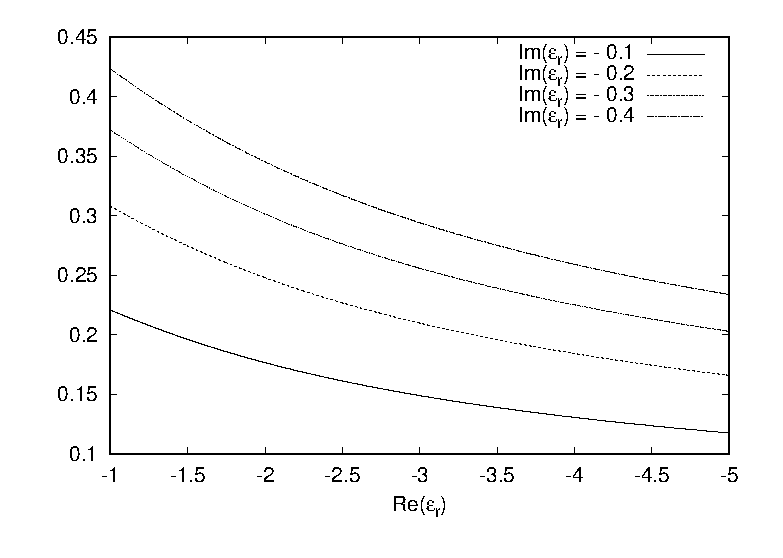
\includegraphics[width=\textwidth]{critical_zeta_vs_real_epsilon_pendry_inf_sup.eps}
\end{subfigure}
%
\begin{subfigure}[b]{0.49\textwidth}
\centering
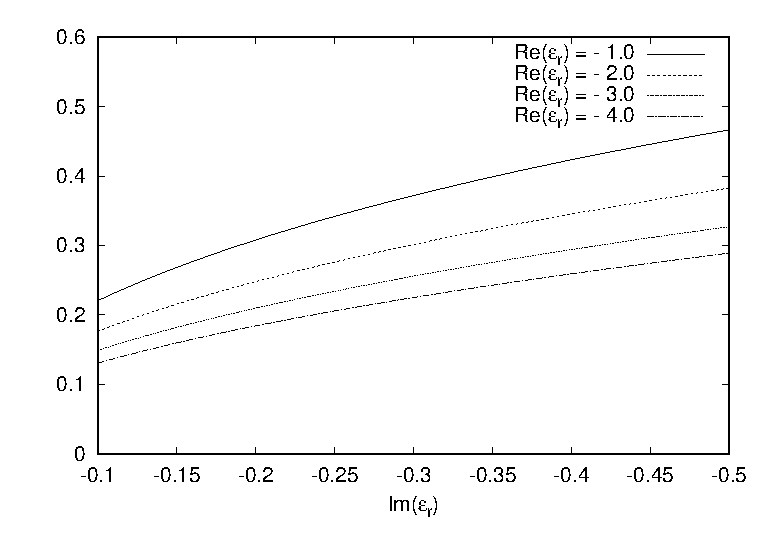
\includegraphics[width=\textwidth]{critical_zeta_vs_imag_epsilon_pendry_inf_sup.eps}
\end{subfigure}
\caption{The magnitude of $\zeta_0$ below which the condition (10) is satisfied as a function of $Re(\varepsilon_r)$ or $Im(\varepsilon_r)$ for media in Kraft et al.
The plot is for real $\zeta_0$ negative values of  $Re(\varepsilon_r)$ or $Im(\varepsilon_r)$ and the material is taken to be non magnetic.}
\label{fi:critical_zeta_vs_epsilonr_inf_sup}
\end{figure}

For checking condition (9) let us represent the constitutive matrices in the alternative form in equations (84), (85) and (86).

\begin{equation} \label{constitutive_kraft_kappa}
\tag{84}
\kappa = \frac{1}{\varepsilon_0\varepsilon_r}
\begin{bmatrix}
1 & 0 & 0 \\
0 & 1 & 0 \\
0 & 0 & \frac{\varepsilon_r\mu_r}{\varepsilon_r\mu_r-\zeta_0^2}
\end{bmatrix}
\end{equation}

\begin{equation} \label{constitutive_kraft_nu}
\tag{85}
\nu = \frac{1}{\mu_0\mu_r}
\begin{bmatrix}
1 & 0 & 0 \\
0 & \frac{\varepsilon_r\mu_r}{\varepsilon_r\mu_r - \zeta_0^2} & 0 \\
0 & 0 & 1
\end{bmatrix}
\end{equation}

\begin{equation} \label{constitutive_kraft_chi_gamma}
\tag{86}
\gamma = -\chi^T = \frac{j\zeta_0c_0}{\varepsilon_r\mu_r-\zeta_0^2}
\begin{bmatrix}
0 & 0 & 0 \\
0 & 0 & 1 \\
0 & 0 & 0
\end{bmatrix}
\end{equation}

The following constants can be evaluated directly using the definitions:

\begin{equation}
\tag{87}
C_{\kappa,d} =  \frac{1}{\varepsilon_0^3}\min(1, \frac{1}{|\varepsilon_r^3(1 - \frac{\zeta_0^2}{\varepsilon_r\mu_r})|}), 
\end{equation}

\begin{equation}
\tag{88}
C_{\nu,d} =  \frac{1}{\mu_0^3}\min(1, \frac{1}{|\mu_r^3(1 - \frac{\zeta_0^2}{\varepsilon_r\mu_r})|}),
\end{equation}

\begin{equation}
\tag{89}
C_{\kappa,r} = \varepsilon_0 \min(1, |\varepsilon_r (1 - \frac{\zeta_0^2}{\varepsilon_r\mu_r})|),
\end{equation}

\begin{equation}
\tag{90}
C_{\nu,r} =  \mu_0 \min(1, |\mu_r(1 - \frac{\zeta_0^2}{\varepsilon_r\mu_r})|), 
\end{equation}

\begin{equation}
\tag{91}
C_{\kappa,s} =  \frac{1}{\varepsilon_0} \max(2, \frac{2}{|\varepsilon_r|}, \frac{1}{|\varepsilon_r|}(1 + \frac{1}{|1 - \frac{\zeta_0^2}{\varepsilon_r\mu_r}|})),
\end{equation}

\begin{equation}
\tag{92}
C_{\nu,s} = \frac{1}{\mu_0} \max(2, \frac{2}{|\mu_r|}, \frac{1}{|\mu_r|}(1 + \frac{1}{|1 - \frac{\zeta_0^2}{\varepsilon_r\mu_r}|})),
\end{equation}

\begin{equation}
\tag{93}
C_{\gamma,s} =  C_{\chi,s} = |\frac{\zeta_0c_0}{\varepsilon_r\mu_r - \zeta_0^2}|. 
\end{equation}

After evaluating these constants, equation (41) gives the criteria for satisfying condition (9).
To get an indication of the trends, let us specialize these evaluations for the case when $\zeta_0$ is real 
and $\mu_r = 1$. 
The dependence of the maximum allowable magnitude of $\zeta_0$ that guarantees condition (9) on $\varepsilon_r$ 
is shown in Figure \ref{fi:critical_zeta_vs_epsilonr_uniqueness}.
For $|Re(\varepsilon_r)| > 1$, the allowable $\zeta_0$ value falls as $|Re(\varepsilon_r)|$ increases and is largely independent of $Im(\varepsilon_r)$.
The maximum permissible $|\zeta_0|$ of $0.4126$ is reached when $Re(\varepsilon_r) = -1$ on the negative side, where as on the positive range of $Re(\varepsilon_r)$ 
the maximum  value is $0.3692$ obtained when $Re(\varepsilon_r) = 1$.   
When $|Re(\varepsilon_r)| < 1$ again the allowable value of $|\zeta_0|$ falls as we move away from $|Re(\varepsilon_r)|=1$ 
and there is some dependence on $Im(\varepsilon_r)$ in this case.

\begin{figure}[H]
\centering
\begin{subfigure}[b]{0.49\textwidth}
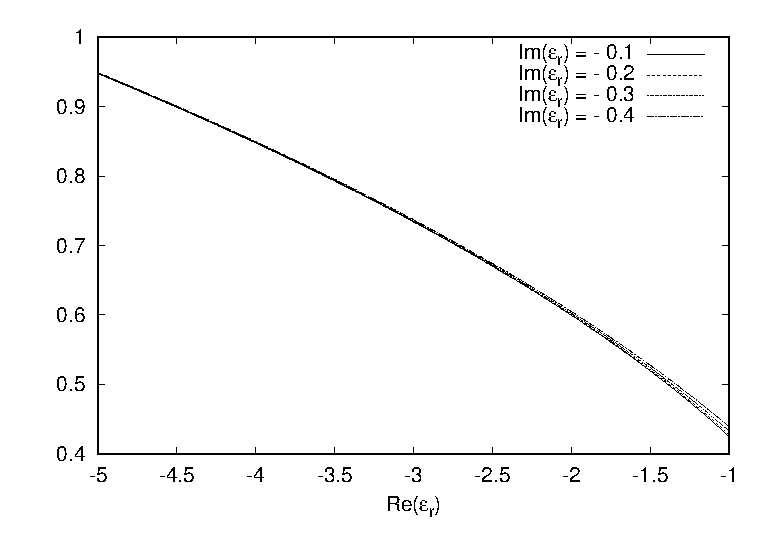
\includegraphics[width=\textwidth]{critical_zeta_vs_real_epsilon_pendry_uniqueness.eps}
\end{subfigure}
%
\begin{subfigure}[b]{0.49\textwidth}
\centering
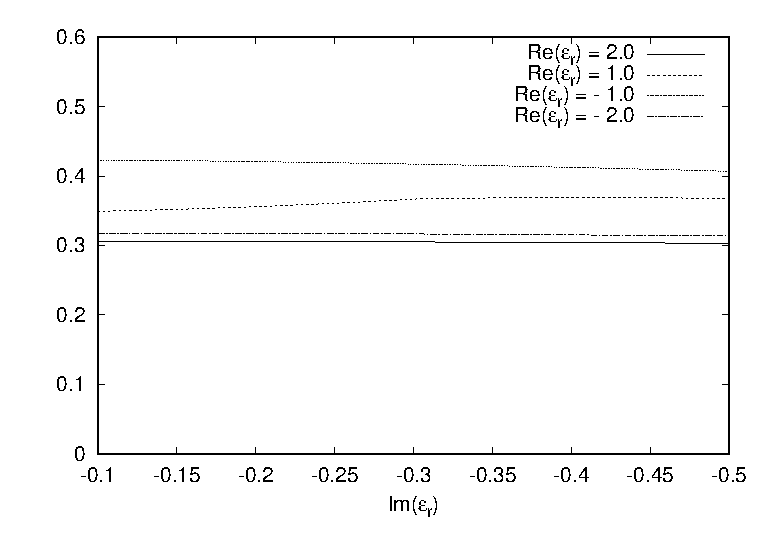
\includegraphics[width=\textwidth]{critical_zeta_vs_imag_epsilon_pendry_uniqueness.eps}
\end{subfigure}
\caption{The magnitude of $\zeta_0$ below which the condition (9) is satisfied as a function of $Re(\varepsilon_r)$ or $Im(\varepsilon_r)$ for media in Kraft et al.
The plot is for real $\zeta_0$ and the material is taken to be non magnetic.}
\label{fi:critical_zeta_vs_epsilonr_uniqueness}
\end{figure}

Let us now turn to a specific numerical example and obtain some results for the fields in the presence of this type of media.
A cube shaped scatterer is considered which is filled with bianisotropic medium of interest and is surrounded by air.
The incident plane wave is travelling along x axis with the electric field polarization along z and having magnitude $1$ $V/m$ 
and the wavelength is $1$ micrometer.
The scatterer is characterized by a cube of side $800$ nm and has $\varepsilon_r = -1 - j0.4$, $\mu_r = 1$ and $\zeta_0 = -0.41$.
This satisfies both conditions required for well posedness since for the given $\varepsilon_r$ and $\mu_r$, 
condition (9) requires $|\zeta_0| < 0.4126$ and  condition (10) requires $|\zeta_0| < 0.4235$.
The numerical domain considered is a cube of side $2$ micrometer and the scatterer is placed at the center of the domain.
The finite element solver is based on Galerkin's method with first order edge elements and with tetrahedral mesh.

\begin{figure}
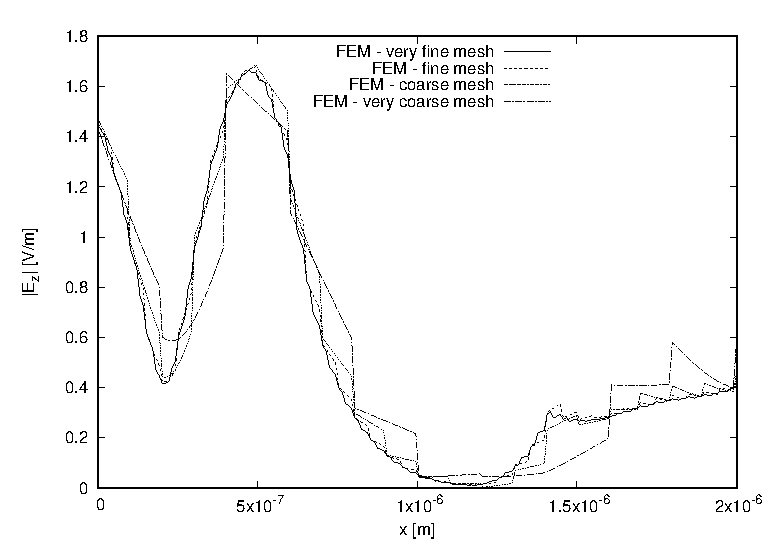
\includegraphics{figure_kraft_pendry_along_x_mag_ez_convergence.eps}
\caption{Convergence of the solution for problem involving medium of Kraft et al.
The magnitude of the $z$ component of the electric field is plotted 
along a line parallel to $x$ axis for four different meshes.}
\label{fi:kraft_pendry_convergence}
\end{figure}

The convergence behaviour of the solution is examined by considering different sizes of the meshes.
The meshing is done by discretizing the domain with small cubes which in turn are divided into six tetrahedra.
The four successive meshes are characterized by cubes of sides $200$ nm, $100$ nm, $50$ nm and $25$ nm which are referred as 
very coarse, coarse, fine and very fine mesh respectively.
The very coarse mesh has 1331 nodes and 6000 elements, coarse mesh has  9261 nodes and 48000 elements, the fine mesh has 68921 nodes and 384000 elements and 
finally the very fine mesh has got 531441 nodes and 3072000 elements.
The result for the $z$ component of the electric field along a line parallel to $x$ axis 
and passing through the center of gravity of the domain ($y = z = 1$ micrometer ) 
is shown in Figure \ref{fi:kraft_pendry_convergence}.
As our theory predicts, the convergence of the solution is obtained and the result with fine mesh is reliable.

To make sense of the bianisotropic effects on the fields due to this kind of media, 
let us compare the solution obtained with that in isotropic case when $\zeta_0 = 0$ but with the same $\varepsilon_r$ and $\mu_r$.
Some of the components of the fields which help to understand such effects are shown in  Figures \ref{fi:kraft_pendry_ez_vs_x} to  \ref{fi:kraft_pendry_ez_vs_z}.
For example there are differences of 10 to 20 percent of incident field in the magnitudes of electric fields which are induced due to the magnetoelectric 
coupling factor $\zeta_0$, as can be seen from the magnitude plots of Figures \ref{fi:kraft_pendry_ez_vs_x} and \ref{fi:kraft_pendry_ez_vs_z}. 
Likewise phases are also affected by the bianisotropy of the medium.
Such results show non negligible influence induced due to the values of $\zeta_0$ that fall within the ranges 
given by our conditions and hence demonstrate the relevance of our theory for the reliability of such solutions.

\begin{figure}[H]
\centering
\begin{subfigure}[b]{0.49\textwidth}
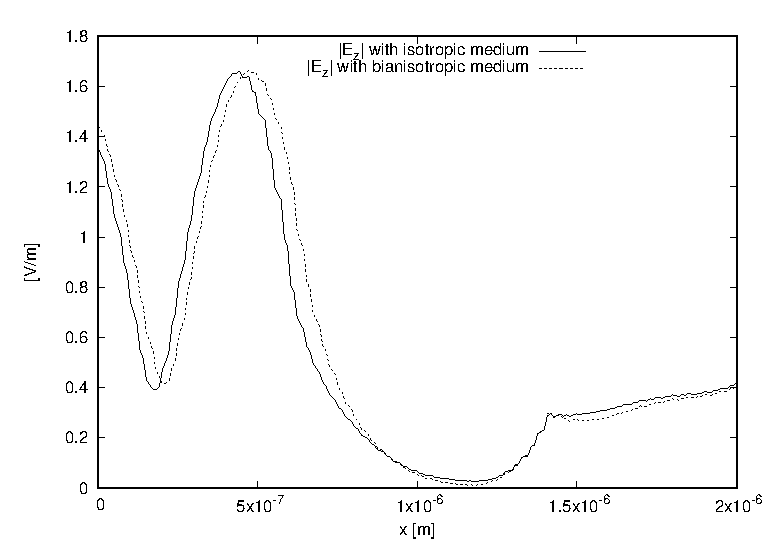
\includegraphics[width=\textwidth]{figure_kraft_pendry_along_x_mag_ez.eps}
\end{subfigure}
%
\begin{subfigure}[b]{0.49\textwidth}
\centering
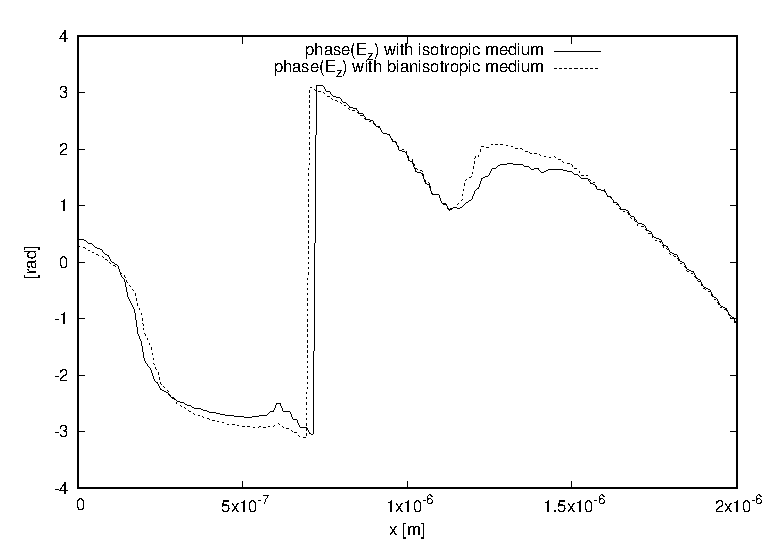
\includegraphics[width=\textwidth]{figure_kraft_pendry_along_x_phase_ez.eps}
\end{subfigure}
\caption{The magnitude and phase of the $z$ component of electric field along a line parallel to $x$ axis 
and passing though the center of gravity of the domain for problem involving medium of Kraft et al. 
The plots for bianisotropic case  using $\zeta_0 = -0.41$ is compared with 
the solution obtained in isotropic case using $\zeta_0 = 0$.}
\label{fi:kraft_pendry_ez_vs_x}
\end{figure}

\begin{figure}[H]
\centering
\begin{subfigure}[b]{0.49\textwidth}
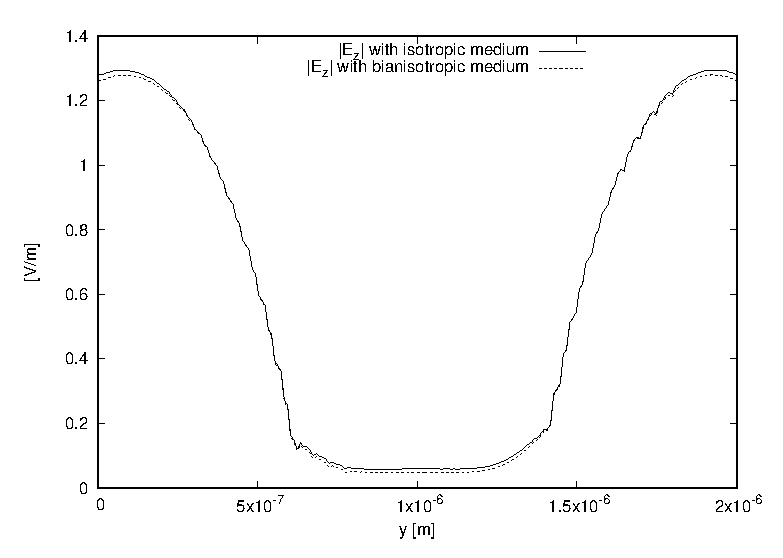
\includegraphics[width=\textwidth]{figure_kraft_pendry_along_y_mag_ez.eps}
\end{subfigure}
%
\begin{subfigure}[b]{0.49\textwidth}
\centering
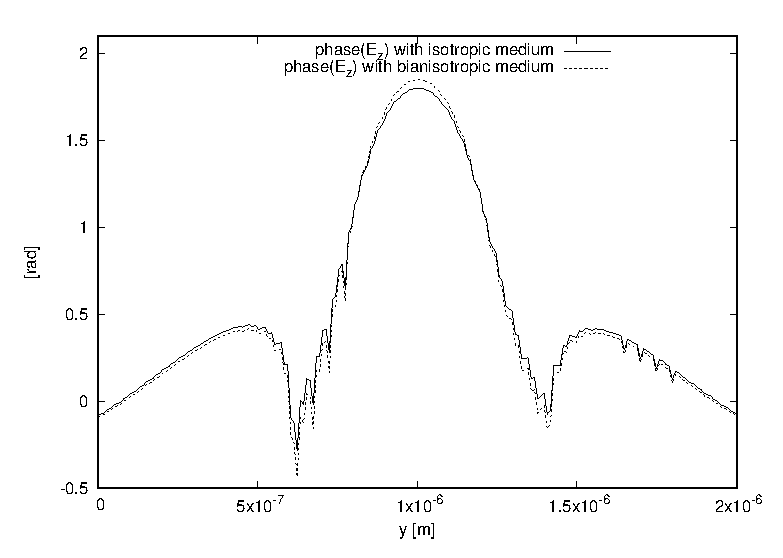
\includegraphics[width=\textwidth]{figure_kraft_pendry_along_y_phase_ez.eps}
\end{subfigure}
\caption{The magnitude and phase of the $z$ component of electric field along a line parallel to $y$ axis 
and passing though the center of gravity of the domain  for problem involving medium of Kraft et al. 
The plots for bianisotropic case using $\zeta_0 = -0.41$ is compared with 
the solution obtained in isotropic case using $\zeta_0 = 0$. }
\label{fi:kraft_pendry_ez_vs_y}
\end{figure}

\begin{figure}[H]
\centering
\begin{subfigure}[b]{0.49\textwidth}
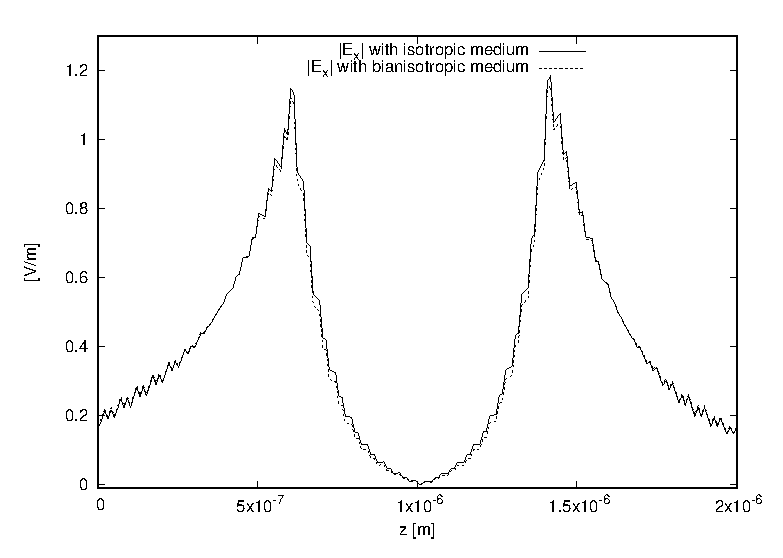
\includegraphics[width=\textwidth]{figure_kraft_pendry_along_z_mag_ex.eps}
\end{subfigure}
%
\begin{subfigure}[b]{0.49\textwidth}
\centering
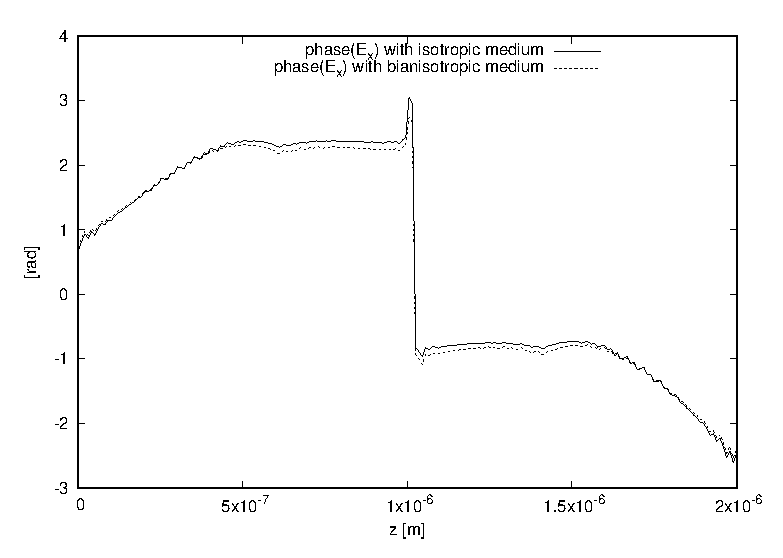
\includegraphics[width=\textwidth]{figure_kraft_pendry_along_z_phase_ex.eps}
\end{subfigure}
\caption{The magnitude and phase of the $x$ component of electric field along a line parallel to $z$ axis 
and passing though the center of gravity of the domain for problem involving medium of Kraft et al. 
The plots for bianisotropic case using $\zeta_0 = -0.41$ is compared with 
the solution obtained in isotropic case using $\zeta_0 = 0$.}
\label{fi:kraft_pendry_ex_vs_z}
\end{figure}

\begin{figure}[H]
\centering
\begin{subfigure}[b]{0.49\textwidth}
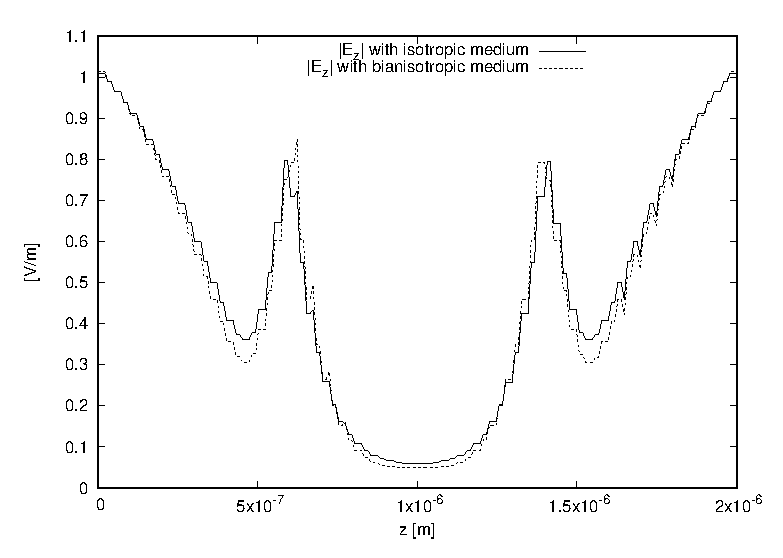
\includegraphics[width=\textwidth]{figure_kraft_pendry_along_z_mag_ez.eps}
\end{subfigure}
%
\begin{subfigure}[b]{0.49\textwidth}
\centering
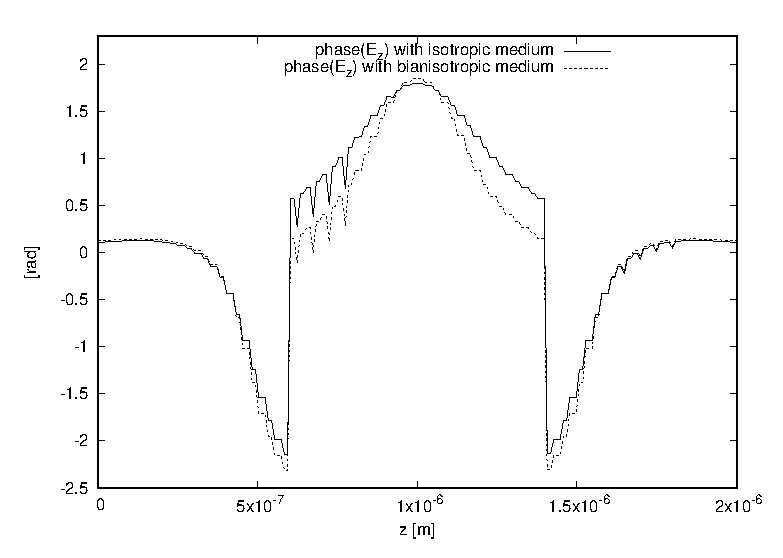
\includegraphics[width=\textwidth]{figure_kraft_pendry_along_z_phase_ez.eps}
\end{subfigure}
\caption{The magnitude and phase of the $z$ component of electric field along a line parallel to $z$ axis 
and passing though the center of gravity of the domain  for problem involving medium of Kraft et al. 
The plots for bianisotropic case using $\zeta_0 = -0.41$ is compared with 
the solution obtained in isotropic case using $\zeta_0 = 0$.}
\label{fi:kraft_pendry_ez_vs_z}
\end{figure}
